\chapter{Theoretical overview}

In this Chapter, the theoretical overview of the Standard Model, flavour physics and \BtoXsgamma will be presented.
It will introduce the main theoretical concepts that are featured in this thesis and provide a theoretical grounding for the experimental analyses performed.
\todo[inline]{section listing here once they are finished}

\section{The Standard Model}

a $SU(3)\times SU(2)\times U(1)$ quantum field theory \cite{Peskin:1995ev}.
Its theoretical framework describes the electroweak and strong force interactions between elementary particles that constitute the world as we know it.
The elementary particles included in the Standard Model can have a half-integer spin (fermions) or integer spin (bosons).
The spin-1 bosons are the mediators of the electromagnetic (photon), weak ($\Wpm$ and $\Z$) and strong interactions (gluon) in the SM.
The spin-0 Higgs boson couples to all massive particles of the Standard Model via the Higgs mechanism \cite{PhysRevLett.13.508}.
The fermions are subsplit into two additional groups, quarks and leptons, which, respectively, can and cannot interact through the strong force.

\section{Flavour physics}

Ongoing...

\section{The decay rate of \texorpdfstring{\BtoXsdgamma}{B->Xsg}}\label{sec:btosgamma_totalrate_theory}

In the Standard Model, $b\ra s$ transitions are mediated by so-called flavour-changing neutral currents.
These processes can only occur through loops mediated by heavy particles.
One of the decay processes used to study these transitions are the so-called rare radiative $b\ra s\g$ and $b\ra d\g$ decays.
Due to colour confinement of the quarks, in reality they manifest as \BtoXsgamma or \BtoXdgamma, where $X_s$ and $X_d$ denote any meson state originating from the $s$ quark hadronisation.
The leading Standard Model diagrams for \BtoXsdgamma (used to collectively identify $X_s$ and $X_d$ states) processes are shown in \Cref{fig:sm_diagrams}.

\todo[inline]{citations here are needed, but I don't know how I want to proceed yet. Maybe this is common knowledge}

\begin{figure}[htbp!]
\resizebox{0.66\textwidth}{!}{
    \subcaptionbox{\label{fig:sm_diagrams}}{
        \begin{tikzpicture}
\begin{feynman}
\vertex (i1){b};
\vertex[right =1.2cm of i1] (a) ;
\vertex[right=0.85cm of a] (b);
\vertex[right=0.85cm of b] (c);
\vertex[right=1.2cm of c] (o1) {s,d};
\vertex[below=2em of c] (g1);
\vertex[right=2em of g1] (o2) {$\gamma$};

\diagram* {
(i1) -- [fermion] (a) -- [boson, edge label =\(W^{\pm}\)] (c) -- [fermion] (o1),
(a) -- [fermion,half left, edge label = \(uct\)] (c),
(b) -- [photon] (o2),
};
\end{feynman}
\end{tikzpicture}

        \begin{tikzpicture}
\begin{feynman}
\vertex (i1){b};
\vertex[right =1.2cm of i1] (a);
\vertex[right=0.85cm of a] (b);
\vertex[right=0.85cm of b] (c);
\vertex[right=1.2cm of c] (o1) {s,d};
\vertex[below=2em of c] (g1);
\vertex[right=2em of g1] (o2) {$\gamma$};

\diagram* {
(i1) -- [fermion] (a) -- [fermion, edge label =\(uct\)] (c) -- [fermion] (o1),
(a) -- [boson,half left, edge label = \(W^{\pm}\)] (c),
(b) -- [photon] (o2),
};
\end{feynman}
\end{tikzpicture}



    }
}
\resizebox{0.33\textwidth}{!}{
\subcaptionbox{\label{fig:bsm_diagrams}}{
    \begin{tikzpicture}
\begin{feynman}
\vertex (i1){b};
\vertex[right =1.2cm of i1] (a) ;
\vertex[right=0.85cm of a] (b);
\vertex[right=0.85cm of b] (c);
\vertex[right=1.2cm of c] (o1) {s,d};
\vertex[below=2em of c] (g1);
\vertex[right=2em of g1] (o2) {$\gamma$};

\diagram* {
(i1) -- [fermion] (a) -- [scalar, edge label =\(H^{\pm}\)] (c) -- [fermion] (o1),
(a) -- [fermion,half left, edge label = \(uct\)] (c),
(b) -- [photon] (o2),
};
\end{feynman}
\end{tikzpicture}

}
}
\caption{\label{fig:b_to_s_gamma_diagrams}
The Feynman diagrams for radiative $b\ra s$ transitions. 
\Cref{fig:sm_diagrams} shows the leading-order Standard Model diagrams, where the $b\ra s$ transition occurs via electroweak loops.
A beyond-Standard Model scenario where this transition is mediated by a charged-Higgs boson particle is shown in \Cref{fig:bsm_diagrams}.
}
\end{figure}

Since \BtoXsdgamma decays proceed via $b\ra s\g$ transitions, they are interesting probes for beyond-Standard-Model (\BSM) particles. 
The leading contributions to these transitions only happen via one-loop diagrams, as seen in \Cref{fig:b_to_s_gamma_diagrams}.
The electroweak loop can get contributions from all the quarks, but is dominated by the much heavier top quark \cite{Mannel:2001vn} as followed by the Glashow-Iliopoulos-Maiani mechanism~\cite{Glashow:1970gm}. 
Furthermore, the masses of possible \BSM weakly-interacting particles that can appear in the loops may be as high as \order{(100~\tev)} \cite{Misiak:2020vlo} which makes studying these decays incredibly appealing.

The decay rate of \BtoXsdgamma is affected by the contributions from weak and strong interactions.
Weak contributions can be calculated perturbatively, however the strong contributions are usually described by effective point-like theories.
In weak decays, including \BtoXsgamma, \textit{Operator Product Expansion} \cite{Peskin:1995ev,Buras:1998raa} is used to derive the effective theory.
It replaces the hadron-binding strong quark interactions and the weak quark interactions mediating $\b\ra\s$ by a single effective vertex.
\todo[inline]{consider adding here sketches}
An effective Lagrangian describing the $\b\to\s\g$ can be written as~\cite{Kaminski:2012eb,Misiak:2015xwa}:
\begin{equation}\label{eq:effective_lagrangian}
    \mathcal{L}_{\mathrm{eff}} = \frac{4G_F}{\sqrt{2}}V_{ts}^*V_{tb}\left[\sum^{8}_{i=1}\mathcal{C}_i(\mu)\mathcal{O}_i(\mu)
                                                + \frac{V^*_{uq}V_{ub}}{V^*_{tq}V_{tb}}\sum^{2}_{i=1}\mathcal{C}_i(\mu)(\mathcal{O}_i(\mu)-\mathcal{O}_i^u(\mu))\right],
\end{equation}
where $G_F$ is the Fermi constant.
The factors $\mathcal{C}_i$, known as \textit{Wilson coefficients}, encode the weak interactions and can be calculated perturbatively.
The other set of operators, $\mathcal{O}_i$ contain the contributions from the strong interactions and are calculated using non-perturbative methods.
The renormalisation scale, $\mu$, is chosen such that strong and weak contributions are separated.
Conventionally, it is set to be of order of the $b$ quark mass $\mu\sim m_b$.

The exact expressions of operators $\mathcal{O}_i$ are given in \Cref{sec:appendix_local_opperators}. 
Coefficients $\mathcal{C}_{3-6}$ have been calculated and shown to be small, therefore the most important contributions arise from $\mathcal{O}_{1,2,7,8}$ \cite{Chetyrkin:1996vx,Misiak:2020vlo}.
Furthermore, the ratio $V^*_{uq}V_{ub}/V^*_{tq}V_{tb}$ is small for the case of $q=s$ \cite{Charles:2015gya}, and the terms including $\mathcal{O}^u_i$ are irrelevant at leading-order calculation of the total decay rate \cite{Misiak:2015xwa}.
Interestingly, the latter point does not hold for $\b\to\d$ case, where additional effects need to be considered due to the contributions from these terms.
In particular, additional non-perturbative uncertainties need to be considered for the Standard Model calculation of the decay rate \cite{Misiak:2015xwa}.
However, for the rest of \Cref{sec:btosgamma_totalrate_theory}, $\b\to\s\g$ decays will be implied unless explicitly stated, as this is the main analysis of the thesis.

The total decay rate of the inclusive \BtoXsgamma is modelled as the rate of its parton decay, taking advantage of the quark-hadron duality.
It is expressed as a sum of a perturbative contribution and non-perturbative correction as \cite{Misiak:2015xwa}:
\begin{equation}\label{eq:btosgammarate_nonp}
    \Gamma(\bar{B}\ra\X_s\g) = \Gamma(b\ra s\g) + \delta\Gamma_{\mathrm{non-p.}},
\end{equation}
$\Gamma(b\ra s\g)$ is the perturbatively calculable rate of $b$ quarks decaying into charmless partons, and $\delta\Gamma_{non-p.}$ is the non-perturbative contribution arising outside of local operator product expansion.
The non-perturbative effects arise from the so-called resolved photon contributions.
These contributions are a result of the photon coupling directly to partons instead of the effective weak interaction vertex.
As long as an appropriately low photon energy threshold (in the decaying $B$ meson frame), \EB, is chosen, the non-perturbative effects in \Cref{eq:btosgammarate_nonp} can be considered smaller as they `average out' over the spectrum.
However, due to contributions from $\ccbar$ resonances at low-\Egamma, it is conventionally chosen at $\Egamma>1.6~\gev$ \cite{Misiak:2009nr}.
Until recently, a 5\% uncertainty was attached to this assumption \cite{Benzke:2010js}. 
However, recent developments in understanding the non-perturbative effects \cite{Gunawardana:2019gep} led to an improved treatment of the associated uncertainties \cite{Misiak:2020vlo}.
The origin of this contribution will be further discussed with the differential decay rate in \Cref{sec:btosgamma_spectrum_theory}.
It will also be seen that the threshold for \EB is motivated also from the experimental side, as large background-process contamination is present in the low-\EB region.

Using operator product expansion, one can calculate the matrix element $|\mel*{s\g}{\mathcal{L}_{\mathrm{eff}}}{b}|^2$ and integrate it from chosen energy threshold, $\Egamma>E_0$. 
Then the perturbative decay rate can be written as \cite{Misiak:2020vlo}:
\begin{equation}\label{eq:theory_decay_rate}
    \Gamma(b\ra\s\g) = \frac{G^2_F m_{\mathrm{b}}^5 \alpha_{\mathrm{em}}}{32\pi^4}|V_{ts}^*V_{tb}|^2\sum_{i,j}^8C^{\mathrm{eff}}_{i}(\mu_b)C^{\mathrm{eff}}_{j}(\mu_b)\hat{G}_{ij}(E_0,\mu_b),
\end{equation}
where $m_{\mathrm{b}}$ is the $b$-quark pole mass, $\alpha_{\mathrm{em}}$ is the fine-structure constant.
The $C_{i}^{\mathrm{eff}}(\mu_b)$ coefficients represent effective Wilson coefficients \cite{Buras:1993xp} that are renormalisation-scheme independent and defined through linear combinations of the Wilson coefficients of \Cref{eq:effective_lagrangian}.
Finally, the functions $\hat{G}_{ij}$ encapsulate the terms describing the interference between operators $\mathcal{O}_{i,j}$, which arise in the squared matrix element.
As already mentioned before, the dominant terms arise from a handful of local operators and the combined efforts to calculate this have brought \BtoXsgamma theoretical estimates to the next-to-next-to-leading order precision.
The dominant functions $\hat{G}_{77}$ \cite{Asatrian:2006rq}, $\hat{G}_{78}$ \cite{Asatrian:2010rq}, $\hat{G}_{(1,2)7}$ \cite{Boughezal:2007ny,Misiak:2020vlo} have been evaluated.
Contributions from $\hat{G}_{(1,2,8)8}$ \cite{Ferroglia:2010xe,Misiak:2010tk} have also been calculated.
In fact, as the calculations have already reached next-to-next-to-leading order precision, even contributions involving $\mathcal{O}_{i}^u$ are accounted \cite{Huber:2014nna}.
The mixing of $\mathcal{O}_{1-6}\to\mathcal{O}_8$ has been also described \cite{Czakon:2006ss}. 
Some of the next-to-next-to-leading order corrections depend on the mass of the charm quark.
However, as the evaluation of such corrections at the physical mass of the charm quark is complicated, the mass is interpolated between $m_c=0$ and $m_c\gg m_b$ \cite{Misiak:2019ccp}.

\Cref{eq:theory_decay_rate} contains a 5th power dependance on the ill-defined pole-mass of the $b$~quark.
Furthermore, uncertainties arising from the CKM matrix element determination also directly enter the calculation.
In order to minimise the uncertainties related to these values, the calculation of \btosgamma decay rate is usually normalised to the semi-leptonic decay rate $b\rightarrow u\ell\nu$.
An alternative choice would be the experimentally more attainable $b\rightarrow c\ell\bar{\nu}$. 
However using the charmless decay rate, allows to separate the $m_c$ determination problem from the problem of calculating higher-order corrections.
In doing so, the decay rate ratio is expressed as \cite{Gambino:2001ew}:
\begin{equation}
    \frac{\Gamma(\b\to\s\g)_{\Egamma>E_0}}{|V_{cb}/V_{ub}|^2 \Gamma(\b\to\u e\nub)} = \left|\frac{V_{ts}^*V_{tb}}{V_{cb}}\right|^2 \frac{6\alpha_{\mathrm{em}}}{\pi}P(E_0).
\end{equation}
Here $P(E_0)$ denotes the perturbatively calculable contribution. 
Replacing $b\ra B$, as seen with \Cref{eq:btosgammarate_nonp}, required the introduction of a non-perturbative correction, $N(E_0)$:

\begin{equation}\label{eq:normalised_br}
    \frac{\Gamma(\BtoXsgamma)_{\Egamma>E_0}}{\Gamma(\B\to X_c\ell\nu_\ell)} = \frac{\mathcal{B}(\BtoXsgamma)_{\Egamma>E_0}}{\mathcal{B}(\B\to X_c\ell\nu_\ell)} = \left|\frac{V_{ts}^*V_{tb}}{V_{cb}}\right|^2\frac{6\alpha_{\mathrm{em}}}{\pi C}[P(E_0)+N(E_0)].
\end{equation}
The additional semileptonic phase-space factor:
\begin{equation}
    C = \left|\frac{V_{ub}}{V_{cb}}\right|^2 \frac{\Gamma(\B\to X_ce\bar{\nu})}{\Gamma(\B\to X_ue\bar{\nu})},
\end{equation}  
accounts for the choice to use the $B\rightarrow X_c\ell\bar{\nu}$ as a normalisation channel for the total-decay rate. 
It is determined using the experimental value of $\B\to X_c \ell\bar{\nu}$, which has a large branching fraction and is known precisely experimentally \cite{Alberti:2014yda,Workman:2022ynf}.
This choice is preferrable compared to the $|V_{ub}|$-supressed and more model-dependant $\B\to X_u\ell\bar{\nu}$.

At leading order, where non-perturbative effects are disregarded, effects from $\mathcal{C}_{2,7,8}$ are most important and this can be expressed in a compact form \cite{Buras:1993xp}:
\begin{equation}\label{eq:total_decay_rate_leading_order}
    \frac{\mathcal{B}(\BtoXsgamma)}{\mathcal{B}(\B\to X_c\ell\nu_\ell)} = \left|\frac{V_{ts}^*V_{tb}}{V_{cb}}\right|^2\frac{6\alpha_{\mathrm{em}}}{\pi C}|C_{7}^{(0)\mathrm{eff}}(\mu)|^2.
\end{equation}
Here $C_{7}^{(0)\mathrm{eff}}(\mu)$ is the effective leading-order Wilson coefficient which was briefly introduced before.
At leading-order, it takes the form:
\begin{equation}\label{eq:effective_c7}
    C_{7}^{(0)\mathrm{eff}}(\mu) = \eta^{16/23}\mathcal{C}^{(0)}_7(\mu) + \frac{8}{3} \left(\eta^{14/23}-\eta^{16/23}\right)\mathcal{C}^{(0)}_8(\mu) + \mathcal{C}^{(0)}_2(\mu) \sum_i^8h_i\eta^{a_i}.
\end{equation}
The Standard Model coefficients $C_{2,7,8}^{(0)}$ are expressed in terms of $x=(m_t/M_W)^2$:
\begin{align}
    \begin{split}
    C_2^{(0)}(M_W) &= 1\\
    C_7^{(0)}(M_W) &= \frac{3x^3-2x^2}{4(x-1)^4}\ln x + \frac{-8x^3-5x^2+7x}{24(x-1)^3}\\
    C_8^{(0)}(M_W) &= \frac{-3x^2}{4(x-1)^4}\ln x + \frac{-x^3+5x^2+2x}{8(x-1)^3}\\
    \end{split}
\end{align}
The coefficient $\eta$ is expressed as $\eta=\alpha_s(M_W)/\alpha_s(\mu)$, whereas $h_i$ and $a_i$ are the eigenvalues of the scheme-independent anomalous dimension matrix $\gamma^{(0)\mathrm{eff}}$, which can be found defined in the Appendix A of Ref. \cite{Buras:1993xp}.
The matrix $\gamma^{(0)\mathrm{eff}}$ governs the leading order QCD corrections to $\b\ra\s\g$ and its elements appear in the renormalisation group equation of the effective Wilson coefficients.

Here it is interesting to look at the \Cref{eq:effective_c7} in more detail. 
In the absence of QCD effects one has $\eta=1$, therefore the \BtoXsgamma decay would be governed solely by the photonic dipole exchange.
However, in the Standard Model, the additional terms lead to a QCD-enhancment of the decay.
To illustrate, when \Cref{eq:effective_c7} is evaluated explicitly:

\todo[inline]{I have to correct these coefficients, probably best according to page 186 of \cite{Buras:1998raa}}

\begin{align}
    \begin{split}
        C_7^{(0)\mathrm{eff}}(M_W) &= 0.689 \cdot C_7^{(0)}(M_W) + 0.087 \cdot C_8^{(0)}(M_W) - 0.161 \cdot C_2^{(0)}(M_W)  \\ 
                          &= 0.689 \cdot (-0.161) + 0.087 \cdot (-0.086) - 0.161\\
                          &= -0.280, \\
    \end{split}
\end{align}
it is clear that the additive QCD two-loop contributions enhance the rate significantly.
Also notable is the fact that the multiplicative QCD correction in the first term suppresses the decay rate, but at a smaller scale than the additive corrections.


\todo[inline]{I could change $M_W$ to $\mu_0$ because it doesnt matter what scale is there I think idk}
% \todo[inline]{I hate this part, need to rethink}

To go beyond the leading-order approximation, one has to take into account the full form of \Cref{eq:normalised_br}.
A sketch of the next-to-leading order can be found in Ref.\cite{Gambino:2001ew}, whereas the most up-to-date total decay rate calculation is describes in Ref.\cite{Misiak:2020vlo} and references therein.
A detailed look of the higher-order calculation of the total \BtoXsgamma decay rate is beyond the scope of this thesis, but such calculations can be followed up in the references already introduced in this chapter and references therein. 
Ref.\cite{Misiak:2020vlo} also includes the most up-to-date estimation of the total decay rate of \BtoXsgamma in the Standard Model:
\begin{equation}
    \mathcal{B}(\BtoXsgamma) = (3.40\pm 0.17) \times 10^{-4}.
\end{equation}
The uncertainties going into the value arise from unevaluated higher-order effects, the necessity to perform an interpolation in $m_c$, and a parametric uncertainty that also encodes the non-perturbative effects.
The first two amount to $3\%$ each, whereas the last is considered at $2.5\%$. 
This amounts to a total uncertainty of, approximately, 4.9\%.
For significant accuracy improvements in the future, higher-order calculations will not be sufficient alone.
It is necessary to remove the dependance on $m_c$ interpolation and improve the treatment of the parametric uncertainties (non-perturbative effects) to go below the $\sqrt{3^2+2.5^2}\approx3.9\%$ uncertainty.

While this value is sufficient to compare the current experimental and theoretical predictions (see Chapter XX), the input from Belle II will reduce the experimental uncertainty below that of the theoretical prediction.
\todo[inline]{experimental status add here or maybe just snowmass citation}

\section{The photon energy spectrum of \texorpdfstring{\BtoXsdgamma}{B->Xsg}}\label{sec:btosgamma_spectrum_theory}

It was already briefly discussed (when introducing \Cref{eq:btosgammarate_nonp}) that theoretical and experimental evaluations of the total \BtoXsgamma decay rate employ a photon-energy threshold.
The non-perturbatve effects that occur at different energy scales compared to the effective $b\ra\s\g$ transition can be integrated out in a treatment of the total decay rate.
However, the choice of a lower-threshold spoils this approximation and introduces non-perturbative corrections.
When considering the photon-energy spectrum, these effects directly manifest as differences in the shape of the spectrum.

At lowest order, $b\ra\s(\d) \g$ is a two-body decay, which means that the decay rate peaks near to the kinematic limit equal to half the \B-meson mass, $m_B/2\gsim E_{\g}$.
Higher-order effects, such as gluonstrahlung, and the Fermi motion of the $b$ quark within the $B$ meson, smear the distribution.
The necessity to account for all of these effects occuring at different energy-scales motivates the use of soft-collinear effective-theory to describe \BtoXsgamma photon-energy spectrum \cite{Neubert:2004qw,Ligeti:2008ac}.
It allows to factorise different contributions to the decay rate, $d\Gamma$, into terms originating from effective hard-interaction vertices, collinear particles and soft particle:
\begin{equation}\label{eq:differential_decay_rate_SCET}
    d\Gamma \propto \mathcal{H} \times \mathcal{J} \otimes \mathcal{S}.
\end{equation}
The $\mathcal{H}$, $\mathcal{J}$, $\mathcal{S}$ represent the hard, jet and hadronic-soft functions, respectively, with $\otimes$ symbolising convolution between the two terms.
Importantly, the $\mathcal{S}$ can be further factorised into a partonic soft-function, $\mathcal{S}_{\mathrm{partonic}}$, and a non-perturbative \textit{shape-function}, $\mathcal{F}$:

\begin{equation}\label{eq:factorisation}
    \mathcal{S} = \mathcal{S}_{\mathrm{partonic}} \otimes \mathcal{F},
\end{equation}
which means that the application of SCET is fully capable to separate perturbative and non-perturbative contributions in the differential decay-rate of \BtoXsgamma.
This is shown graphically in \Cref{fig:xsgamma_theory_sketches}, which sketch out the leading-order, perturbative and non-perturbative effects in describing the \BtoXsgamma spectrum.

Due to the larger \BtoXsgamma decay rate and overall smaller background-process rate, experimental values have the highest precision around the peak region.
However, from the theory side, the peak part is mostly governed by the non-perturbative effects, encoded within the shape function \cite{Ligeti:2008ac}.
The shape function encodes the $b$-quark residual-momentum distribution within the $B$-meson. 
Therefore, reliable theoretical description of the shape-function is critical to make sensible experimental and theoretical comparisons of the photon-energy spectrum. 

\begin{figure}[htbp!]
    \subcaptionbox{\label{fig:theory_to_experiment}}{
        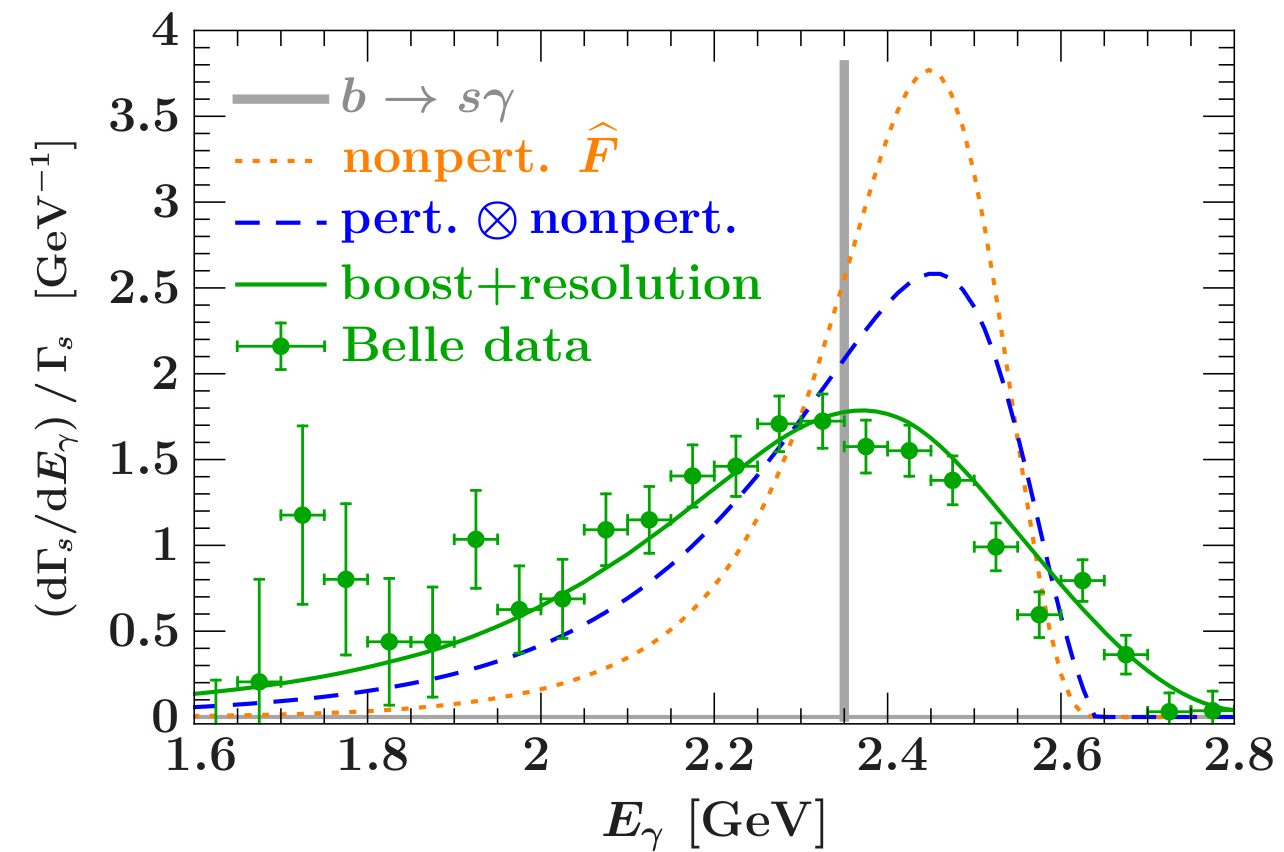
\includegraphics[width=0.5\textwidth]{figures/theory/xsgamma_theory_to_experiment.png}
    }
    \subcaptionbox{\label{fig:theory_ingredients_schematic}}{
        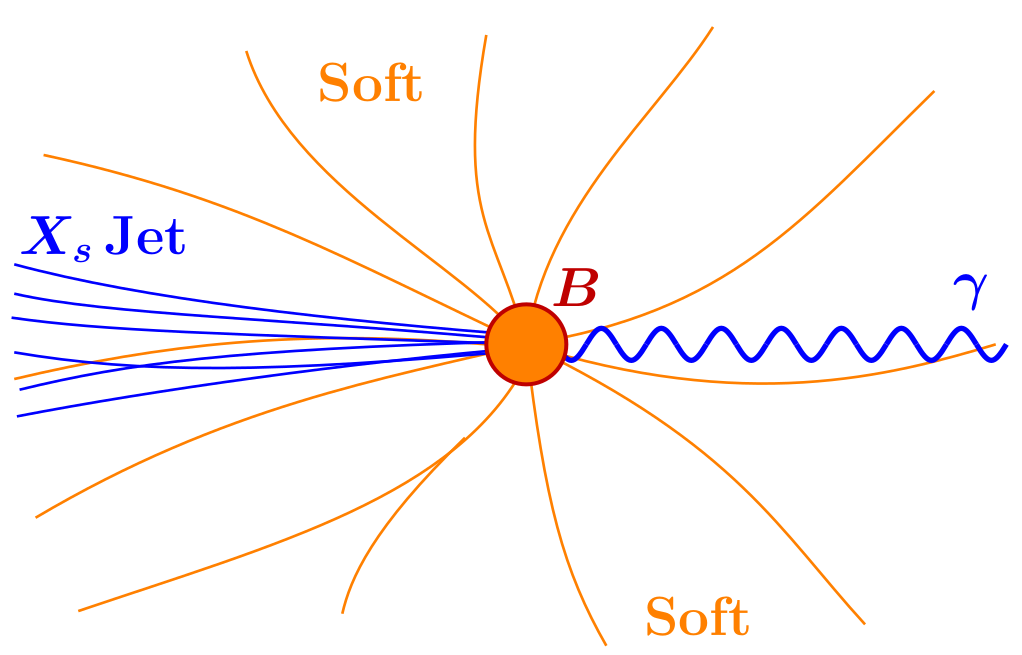
\includegraphics[width=0.5\textwidth]{figures/theory/xsgamma_theory_components.png}
    }
    \caption{\label{fig:xsgamma_theory_sketches} 
    The schematic representation of the theoretical \BtoXsgamma spectrum components and the comparison of them in data.
    Note that the figures are presented only for illustration purposes and do not represent a highly-accurate depiction.
    \Cref{fig:theory_to_experiment} represent the leading-order $\delta$ function spectrum, the non-perturbative shape-function effects, and the convolution of these effects with the perturbatively calculable ones.
    It also includes the experimental effects, such as finite detector resolution.
    \Cref{fig:theory_ingredients_schematic} illustrates the origin of perturbative and non-perturbative effects in a \BtoXsgamma decay.
    Credit to Dr.Frank Tackmann.}
\end{figure}

An additional motivation to study the shape function is the fact that such function is a universal property of the $B$ meson at leading order in $1/m_b$ \cite{Neubert:1993um,Bigi:1993ex}.
This allows to extract the functional form by a precise experimental determination of the \BtoXsgamma spectrum and use it to improve the precision of other measurements.
For example, in the measurement of the $|V_{ub}|$ using $B\rightarrow X_u \ell \bar{\nu_{\ell}}$ decays suffers from orders-of-magnitude larger backgrounds from $B\rightarrow X_c \ell \bar{\nu_{\ell}}$ in most phase-space regions.
The regions where this background is kinematically-forbidden, the theoretical predictions are dependant on these non-perturbative shape functions.
The extracted inputs from \BtoXsgamma could then be used to predict the $B\rightarrow X_u \ell \bar{\nu_{\ell}}$ spectra.
This is an important relation which could lead to a model-independent evaluation of the $|V_{ub}|$ element \cite{Neubert:1993um}.

Let's consider \Cref{eq:differential_decay_rate_SCET,eq:factorisation} in a bit more detail.
Following the treatment of Ref.~\cite{Ligeti:2008ac}, the differential decay rate takes the form:

\begin{equation}\label{eq:differential_decay_simba}
    \frac{d\Gamma}{dE_{\gamma}} = 2\frac{G_F^2\alpha_{\mathrm{em}} m_b^5}{32\pi^4}|V_{ts}V_{tb}^*|^2 \mathcal{H}(x, \mu) \times \int dk \mathcal{P}(m_b, x - k, \mu_i) \mathcal{F}(k) + \order\left(\frac{\Lambda_{\mathrm{QCD}}}{m_b}\right),
\end{equation}
where $x=m_B-2\Egamma$, $\mathcal{P}$ is used to denote the perturbatively calculable $\mathcal{J}\times\mathcal{S_{\mathrm{partonic}}}$ and the symbolic convolution has now been replaced by an integration over a dummy-momentum $k$.
The higher order corrections introduce additional shape-functions, but are suppressed by a factor of $1/m_b$ \cite{Neubert:2002yx}.
Generally, $\mathcal{H}$ and $\mathcal{P}$ is calculable in perturbation theory (see Appendix A of \cite{Ligeti:2008ac}).
$\mathcal{H}$ is directly expressed in terms of the effecive Wilson coefficient $\mathcal{C}_7^{\mathrm{eff}}$. 
Moreover, at lowest-order in perturbation theory $\mathcal{P}$ can be expressed as a delta function:

\begin{equation}
    \mathcal{P}(m_B,k,\mu) = \delta(k) + \mathcal{O}(\alpha_s),
\end{equation}
and therefore integrating out the momentum $k$:
\begin{equation}\label{eq:integrated_egamma}
    \frac{d\Gamma}{d\Egamma} \propto |C_7^{\mathrm{eff}}|^2 \mathcal{F}(x).
\end{equation}
This shows, as stated before, that the peak region (close to $m_b/2$) is governed by the shape-function.
In that case $|C_7|$ is the normalisation of the spectrum.
The shape function can be formally expanded in its moments as \cite{PhysRevD.50.2037,Ligeti:2008ac}:
\begin{equation}\label{eq:shape_function_expansion}
    \mathcal{F}(x) = \sum_n \frac{1}{n!} A_n \dv[n]{\delta(x)}{x},
\end{equation}
where 
\begin{equation}\label{eq:moments_of_shape_function}
    A_n = \int dk k^n \mathcal{F}(k).
\end{equation}
The \Cref{eq:moments_of_shape_function} is the expression for the $n$-th moment of the shape function.
In all shape-function based calculations $A_0=1$ is fixed, because the shape-function is normalised.
Note that if one naively neglects $n>1$ terms, the integral over total $\Egamma$ of \Cref{eq:integrated_egamma} would take the form $\Gamma\sim|C_7^{\mathrm{eff}}|^2$, which is consistent with \Cref{eq:total_decay_rate_leading_order}.
Therefore, for total decay-rate calculations (such as the ones sketched in \Cref{sec:btosgamma_totalrate_theory}) it is enough to know the first several moments of the shape function, as the more delicate $\mathcal{F}(k)$ dependance is suppressed by the factorial $n!$ terms.

For example, consider taking only terms up to first order.
In such case, using the definition of an average,
\begin{equation}
    \expval{\Egamma} = \frac{\int d\Egamma \Egamma \dv{\Gamma}{\Egamma}}{\int d\Egamma \dv{\Gamma}{\Egamma}},
\end{equation}
the shape function is directly related to the average of the photon-energy spectrum.
Similarly, the variance (and higher-order moments) contribute if more terms from \Cref{eq:shape_function_expansion} are considered.
As shown in Refs.\cite{Bauer:1997fe,Kapustin:1995fk} (and others) two important relations can be shown to emerge:
\begin{equation}
    \expval{\Egamma} \sim m_b/2+\order(m_b^2); \quad \expval{\Egamma^2}-\expval{\Egamma}^2 \sim \lambda_1/3+\order(m_b^2),
\end{equation}
with the $b$-quark pole-mass, $m_b$, and the residual-momentum caried by the $b$-quark within the $B$ meson, $\lambda_1$.

The form of the shape function is not well-known and non-perturbative, unlike the Wilson coefficients.
Therefore, theoretical and experimental comparisons always lead to modelling-related uncertainties.
There are a number of different works which propose ways to describe it \cite{Benson:2004sg,Lange:2005yw,Andersen:2005mj,Gambino:2007rp,Aglietti:2007ik,Bernlochner:2020jlt}.
For example, Ref. \cite{Andersen:2005mj} describe it based on a technique called dressed gluon exponentiation.
The result of Ref. \cite{Lange:2005yw} provides several functional forms of the shape function, based on the leading-order shape-function that can be extracted from \BtoXsgamma decays.
An interesting analysis by the SIMBA collaboration \cite{Bernlochner:2020jlt} describes a model-independent treatment of the shape function based on \Cref{eq:differential_decay_simba}.
In particular, any chosen shape function is expanded in a complete set of orthonormal basis functions, and can therefore be extracted, together with the normalisation, from a global-fit of available experimental results.
The strength of this approach is a consistent method to combine several experimental inputs for the extraction of the shape function and its moments.

One of the most commonly chosen inclusive \BtoXsgamma models for experimental analyses is known as the Kagan-Neubert model \cite{Kagan:1998ym}.
It provides a next-to-leading order description of the inclusive \BtoXsgamma spectrum. 
In this model, the shape function takes a simple form:
\begin{equation}
    \mathcal{F}(x) = N\left(1-\frac{x}{m_B-m_b}\right)^a\exp{(1+a)\frac{x}{m_B-m_b}}.
\end{equation}
The shape function satisfies the necessary moment constraints through these relations: $A_0=1,A_1 = 0,A_2=-\lambda_1/3$.
The parameter $a$ is also related to $A_2=(m_B-m_b)/(1+a)$.
Therefore, the shape-function can be fully described by two free parameters $m_b$ and $\lambda_1$.
This relatively straightforward relation makes it easy to implement and interpret.
Furthermore, the Kagan-Neubert model is readily available in \texttt{EvtGen} Monte Carlo generator, commonly used by $B$-factories \cite{Ryd:2005zz}.
The \BtoXsgamma inclusive decay is implemented as the \texttt{BTOXSGAMMA} model within the generator. 
These points made it the conventional choice for experimental description of the inclusive-\Egamma spectrum in many of past measurements.

The previous argument may also be used inversely: an accurate experimental measurement of the \BtoXsgamma spectrum, can be used to precisely determine the parameters $m_b$ and $\lambda_1$ (and also higher moments of the shape function).
One such example is the aforementioned SIMBA collaboration result \cite{Bernlochner:2020jlt}.
The evaluated values of $m_b$ and $\lambda_1$ by the SIMBA collaboration from fitting available \BtoXsgamma experimental results are:

\begin{equation}
    m_b^{1S} =4.750~\gev \pm 0.043;  \quad \lambda^{\mathrm{inv}}_1 = -0.210\pm0.083,~\gev^2, 
\end{equation}
where uncertainties are combined fitting, theoretical and parametric.
These results originate directly from experimental-data fits and have slightly-larger than world-average uncertainties.
The superscript $1S$ and the hat on the operator $\lambda$ indicate a renormalisation-scheme that is chosen by the authors.

The works presented in this thesis will use the Kagan-Neubert model to generate the inclusive photon-energy spectrum.
I will use the $m_b$ and $\lambda_1$ values measured by the SIMBA collaboration, as they are extracted from all available experimental evidence, and contain slightly-larger uncertainties making it a safer conservative estimate.
The relations provided in \cite{Ligeti:2008ac} will be used to transform the `$1S$/invisible' scheme to the kinetic-scheme at precision of $\order(\alpha_s^2)$, that can be used in the Kagan-Neubert model.


\section{New-physics opportunities in \texorpdfstring{\BtoXsdgamma}{B->Xsg}}

